\setchapterimage[6cm]{chapter/ship/ship_title_image.jpeg}
\setchapterpreamble[u]{\margintoc}
\chapter{Warships and their operators\protect\footnotemark}
\labch{ship}

\footnotetext{Imperial Japanese Navy battleship Fusō prepares for a review at Yokohama, Japan. \href{https://commons.wikimedia.org/wiki/File:Fuso_Yokohama.jpg}{WikiCommons / 1928 / Public domain}. Kure Maritime Museum (edited by Kazushige Todaka), Japanese Naval Warship Photo Album: Battleships and Battle Cruisers, p. 129.}


This chapter focuses on ships in Russia and in the world. Ships have different purposes, for example: military, civil. Civilian ships are used in a variety of tasks: trucking, fishing, tourism, mineral exploration, rescue work, as well as sports, cultural and other activities. To store a large amount of information about all ships, it is necessary to maintain knowledge bases. One of those knowledge bases is Wikidata. This work is aimed at studying the stored in Wikidata objects describing ships and at evaluating the quality and completeness of their properties and descriptions.


\begin{marginfigure}[0.0cm]
  {
    \setlength{\fboxsep}{0pt}%
    \setlength{\fboxrule}{1pt}%
    \fcolorbox{gray}{gray}{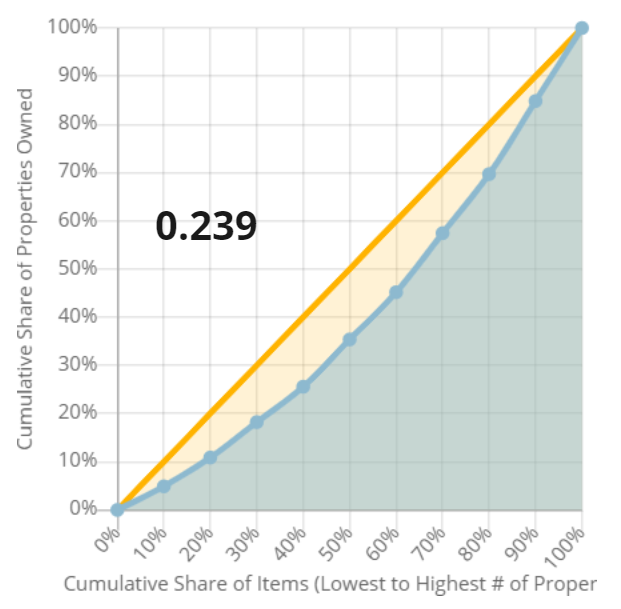
\includegraphics[width=0.9\linewidth]{chapter/ship/Russian_ships_topic_imbalance.png}}
  }
  \caption[Graph of Wikidata objects' completeness]{Graph of \href{https://www.wikidata.org/wiki/Q11446}{ship (Q11446)} Wikidata objects' completeness. Gini coefficient equals 0.239. Data was collected with ProWD.id, 2020. Completeness is not uniform.}%
  \label{fig:prowd_ships-unbalanced}%
\end{marginfigure}

\section{List of ships}

A \href{https://www.wikidata.org/wiki/Q11446}{ship (Q11446)} is a large marine vessel.



Wikidata properties considered in the chapter: 
\begin{itemize}
  \item \href{https://www.wikidata.org/wiki/Property:P31}{instance of (P31)};
  \item \href{https://www.wikidata.org/wiki/Property:P137}{operator (P137)};
  \item \href{https://www.wikidata.org/wiki/Property:P17}{country (P17)};
  \item \href{https://www.wikidata.org/wiki/Property:P607}{conflict (P607)}.
\end{itemize}

Let's build a list of all ships with the script in the listing \ref{lst:list_of_ship_en}


\begin{lstlisting}[ language=SPARQL, caption={List of ships. \num{19820} ships (2017), \num{50681} ships (2020), \num{71203} ships (2021). SPARQL-query: \href{https://w.wiki/vhp}{https://w.wiki/vhp}}, label=lst:list_of_ship_en, texcl]
# List of ships
SELECT ?ship ?shipLabel
WHERE
{
  ?ship wdt:P31 wd:Q11446. # instance of ship
SERVICE wikibase:label {bd:serviceParam wikibase:language "en"}
}
\end{lstlisting}


\begin{marginfigure}[0.0cm]
  {
    \setlength{\fboxsep}{0pt}%
    \setlength{\fboxrule}{1pt}%
    \fcolorbox{gray}{gray}{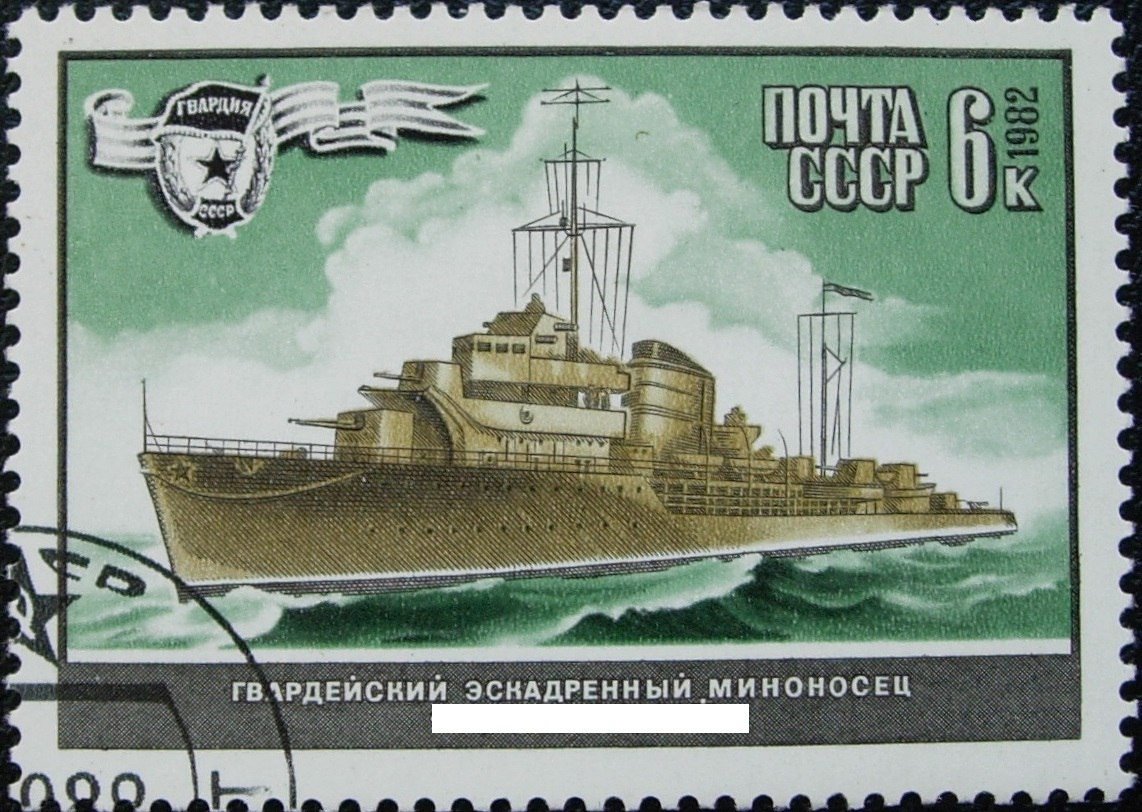
\includegraphics[width=0.92\linewidth]{chapter/ship/Secret_Grem_ship.jpg}}
  }
  \caption[Soviet destroyer project 7]{Postage stamp with a picture of famous Soviet \Wikiref{Gnevny-class destroyer}, USSR, 1982.}%
  \label{fig:quiz_question_ship}%
\end{marginfigure}
  
\begin{lstlisting}[ language=SPARQL, caption={List of ship from Russia, Soviet Union and Russian Empire. \num{107} ships (2017), \num{578} ships (2021). SPARQL-query: \href{https://w.wiki/vuM}{https://w.wiki/vuM}}, label=lst:list_of_ship_ussr_rf_re_en, texcl]
# List of ship from Russia, Soviet Union and Russian Empire
SELECT ?ship ?shipLabel
WHERE
{
  ?ship wdt:P31 wd:Q11446; # instance of ship
        wdt:P137/wdt:P17 ?country. # belongs to country
    
  VALUES ?country {wd:Q34266 # Russian Empire
                   wd:Q15180 # Soviet Union
                   wd:Q159}  # Russia
  SERVICE wikibase:label {bd:serviceParam wikibase:language "en"}
}
\end{lstlisting}

\label{question:ship_1}
\marginnote{The figure \ref{fig:quiz_question_ship} shows the most famous Soviet \Wikiref{Gnevny-class destroyer}, awarded the title of ``Guard'', name it. See answer on page~\pageref{answer:ship_1}.}

The ship \href{https://www.wikidata.org/wiki/Q281147}{Krasin (Q281147)} has the maximum number of properties (34 properties) in WIkidata according to ProWD \sidecite{ProWD_ru_ships}. The ships \href{https://www.wikidata.org/wiki/Q99198666}{Liven (Q99198666)} and \href{https://www.wikidata.org/wiki/Q28155282}{Dispatch (Q28155282)} have the minimym number of properties (5 properties).


\section{Completeness of the Wikidata ships' objects}

Finding the exact number of ships in the world is a difficult task. After all, data about some of them are top secret, some are private vessels and there is no information about them either. Suppose that the total number of ships is about 1.6 millions, as indicated in the vessel database \sidecite{FleetMon}. The script in the listing \ref{lst:list_of_ship_en} showed only \num{71203} records, which makes up only 4.5\% of the total number of ships. 

As for the Russian ships, the actual civil and military fleets includes \num{17657} ships \sidecite{RussianShips}. In 2021 the script in the listing \ref{lst:list_of_ship_ussr_rf_re_en} showed only 578 records, which is only 3.27\% of the total number of Russian ships. 

\label{question:ship_2}
\marginnote[-0.1cm]{Find ships worthy of mention in the Guinness Book, namely: the largest, the longest, the most capacious, etc. See answer on page~\pageref{answer:ship_2}.}

In the first and second cases, there are small percentage of ships in Wikidata, which indicates the incompleteness of the Wikidata. It is also showed by Fig. \ref{fig:prowd_ships-unbalanced}.


\section{Ships objects' properties completeness}

It is required to find ships that participated in any military conflicts. Let's do this with the scipt in the listing \ref{lst:ships_in_conflict_en}.

\begin{lstlisting}[ language=SPARQL, caption={List of ships with countries and war conflicts in English. \num{1400} ships (2017), \num{3567} ships (2021). SPARQL-query: \href{https://w.wiki/vi2}{https://w.wiki/vi2}}, label=lst:ships_in_conflict_en, texcl]
# List of ships with countries and war conflicts
SELECT ?ship ?shipLabel ?countryLabel ?conflict ?conflictLabel
WHERE
{
  ?ship wdt:P31 wd:Q11446;        # instance of ship
        wdt:P137/wdt:P17 ?country;# belongs to country
        wdt:P607 ?conflict.       # engaged in some conflict
SERVICE wikibase:label {bd:serviceParam wikibase:language "en"}
}
\end{lstlisting}

With the serarator ``'';'' in the script in the listing \ref{lst:ships_in_conflict_en} it is possible to extract multiple properties of the same object in one line of code. It this script 3 values were extracted: \href{https://www.wikidata.org/wiki/Property:P31}{instance of (P31)}, \href{https://www.wikidata.org/wiki/Property:P17}{country (P17)} of the \href{https://www.wikidata.org/wiki/Property:P137}{operator (P137)} and \href{https://www.wikidata.org/wiki/Property:P607}{conflict (P607)}. It should be noted that \href{https://www.wikidata.org/wiki/Property:P607}{conflict (P607)} and \href{https://www.wikidata.org/wiki/Q645883}{military operation (Q645883)}, which are part of wars, are different concepts. Wikidata ships can be roughly divided into two types:

\begin{itemize}
  \item \textbf{Objects in which military operations are combined with military conflicts}. For example, object \href{https://www.wikidata.org/wiki/Q4148613}{Soviet destroyer Gremyashchiy} contains 10 wars / battles in field \href{https://www.wikidata.org/wiki/Q180684}{conflict (Q180684)}, see listing \ref{lst:grem_wars}. Such a large number is due to the fact that the ship took part in many \href{https://en.wikipedia.org/wiki/Arctic_convoys_of_World_War_II}{arctic convoys} which are military operations.
  
  \item \textbf{Objects in which military operations are separated from military conflicts}. For example, the participation of the British cruiser \href{https://www.wikidata.org/wiki/Q1565575}{HMS Trinidad (Q1565575)} in the military campaign and in the Arctic convoy are listed as part of World War II with the qualifier\marginnote{For more information about the qualifiers see: \href{w.wiki/w7n}{w.wiki/w7n}} \href{https://www.wikidata.org/wiki/Property:P1012}{including (P1012)}. Thus, in the Wikidata, this cruiser has one war/battle.
\end{itemize}

Thus, the first type of object contains more \href{https://www.wikidata.org/wiki/Property:P607}{conflicts (P607)} than the second type. The ships of the first type will display more wars/battles than the second type. 
%But in this case, the operation \href{https://www.wikidata.org/wiki/Q682409}{Siege of Odessa (Q682409)} will stand alongside \href{https://www.wikidata.org/wiki/Q362}{World War II (Q362)}, although it is part of this war. In this situation, the output data will not be accurate.

\begin{lstlisting}[ language=SPARQL, caption={War conflicts with \href{https://www.wikidata.org/wiki/Q4148613}{destroyer Gremyashchiy} and \href{https://www.wikidata.org/wiki/Q1565575}{HMS Trinidad (Q1565575)}. \num{10} and \num{1} conflicts were found respectively, 2021. SPARQL-query: \href{https://w.wiki/vuE}{https://w.wiki/vuE}}, label=lst:grem_wars, ]
# List of military conflicts of the two ships 
SELECT ?ship ?shipLabel ?conflict ?conflictLabel
WHERE
{
  VALUES ?ship {wd:Q4148613   # Soviet destroyer Gremyashchiy
                wd:Q1565575}  # United Kingdom's HMS Trinidad
  ?ship wdt:P607 ?conflict.   # conflict
SERVICE wikibase:label {bd:serviceParam wikibase:language "en"}
}
\end{lstlisting}

\label{question:ship_3}
\marginnote{Find images of ships that have been used in a movie. If there are no such, then those ships, about which the books were written. See answer on page~\pageref{answer:ship_3}.}

Also, let's build list of conflict and ships of Russian Empire, USSR and Russia, with script in the listing \ref{lst:ships_in_conflict_2_en}.

\begin{lstlisting}[ language=SPARQL, caption={List of ships with countries and war conflicts in English. \num{105} ships (2017), \num{86} ships (2020), \num{82} ships (2021) were found. SPARQL-query: \href{https://w.wiki/vuP}{https://w.wiki/vuP}}, label=lst:ships_in_conflict_2_en, texcl]
# List of ship with countries and war conflicts
SELECT ?ship ?shipLabel ?countryLabel ?conflict ?conflictLabel
WHERE
{
  ?ship wdt:P31 wd:Q11446;        # instance of ship
        wdt:P137/wdt:P17 ?country;# belongs to country
        wdt:P607 ?conflict.       # engaged in some conflict
  
  VALUES ?country {wd:Q34266 # Russian Empire
                   wd:Q15180 # Soviet Union
                   wd:Q159}  # Russia
SERVICE wikibase:label {bd:serviceParam wikibase:language "en"}
}
\end{lstlisting}

Note that not all of the ships in the script in Listing \ref{lst:ships_in_conflict_2_en} are associated with Russia, the USSR, or the Russian Empire. For example, there is \href{https://www.wikidata.org/wiki/Q653477}{Kasato Maru (Q653477)}. This ship belonged to Russia in 1900-1905, belonged to Japan since 1906. It means that the same ship may be owned by different operators in different periods of the time.


\section{Museum ships around the world}
\href{https://www.wikidata.org/wiki/Q575727}{Museum Ship (Q575727)} is a ship that houses a museum exhibition dedicated to the history of the ship. Such ships are used for educational and memorial purposes. The ship's participation in the \href{https://www.wikidata.org/wiki/Q180684}{conflict (Q180684)} may lead to the creation of a museum ship in memory of past events.

Let's build a graph of museum ships and the countries in which these ships are located. The vertices of the graph are \href{https://www.wikidata.org/wiki/Q6256}{countries (Q6256)} and \href{https://www.wikidata.org/wiki/Q575727}{museum ships (Q575727)}. The edge between a ship and a country means that the ship is in that country. And the edge between the two countries means that there were conflicts between these countries, the number of which is equal to the weight of the edge. The script in listing \ref{lst:museum_graph} builds this graph according to the rules described above.


\marginnote[7.0cm]{This FILTER function deletes selfloops and double edges between countries.}
\marginnote[12.0cm]{Here we need to use the `` p:/ps:'' because of multiple values in the property \href{https://www.wikidata.org/wiki/Property:P31}{instance of (P31)} for country. See more information in section~\ref{RussiaNotCountryPPS} on page~\pageref{RussiaNotCountryPPS}.}
\begin{lstlisting}[ language=SPARQL, caption={The graph of museum ships and the countries in which these ships are located. 117 vertices are found (2021). SPARQL-query: \href{https://w.wiki/wBA}{https://w.wiki/wBA}}, label=lst:museum_graph, ]
#defaultView:Graph    
SELECT ?v1 ?v1Label ?v2 ?v2Label ?edgeLabel ?img 
WHERE {
  {SELECT ?c ?cLabel ?v1 ?v1Label ?v2 ?v2Label 
                     (STR(COUNT(?c)) as ?edgeLabel) 
    WHERE
    {
    VALUES ?cTypes 
          {wd:Q180684 # conflict
           wd:Q831663 # military campaign
           wd:Q645883 # military operation
           wd:Q198    # war
          } 
    ?c wdt:P31 ?cTypes.
    ?v1 wdt:P31 wd:Q6256. ?v2 wdt:P31 wd:Q6256. # country
    ?c wdt:P710 ?v1, ?v2. # in war
    FILTER (?v1 != ?v2 && STR(?v1) < STR(?v2)) 
  SERVICE wikibase:label {bd:serviceParam wikibase:language "en"}
  }
  GROUP BY ?c ?cLabel ?v1 ?v1Label ?v2 ?v2Label
  }
  UNION
  {SELECT DISTINCT ?v1 ?v1Label ?v2 ?v2Label ?img
   WHERE
   {
      ?v2 wdt:P31 wd:Q575727. # museum ship
      {?v2 p:P17 [ps:P17 ?v1]} UNION # ?v2 has country ?v1
      {
        ?v2 wdt:P131 ?loc.      # in ?loc
        ?loc p:P17 [ps:P17 ?v1].# ?loc in country ?v1
      }
      OPTIONAL {?v2 wdt:P18 ?img}
  SERVICE wikibase:label {bd:serviceParam wikibase:language "en"}
   }
 }
}
\end{lstlisting}

From a fragment of the graph in figure \ref{fig:museum_graph} it can be seen that the museum ships mostly belong to Germany, the USA and Australia. This ``correlation'' is quite logical, since these countries have a long history, for which they have participated in many conflicts. Also, these countries have access to the sea, which historically determines the presence of a fleet.

\begin{figure*}[ht]
  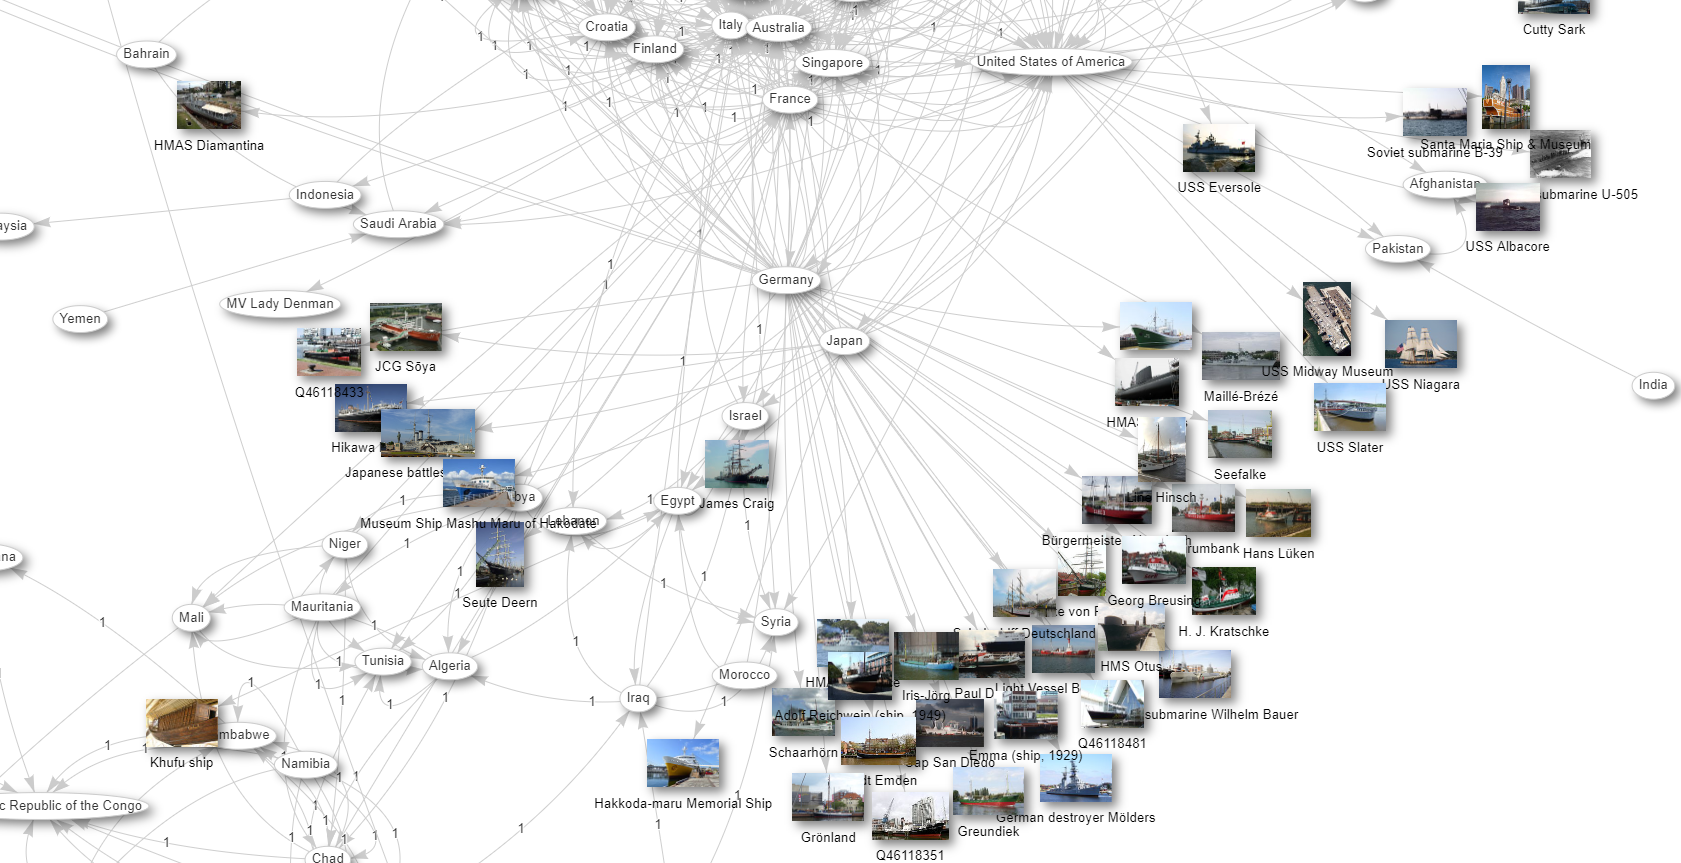
\includegraphics[width=0.9\linewidth]{chapter/ship/museum_graph.png}
  \caption[Graph of countries and museum ships]{Fragment of the graph of countries, museum ships and conflicts, built via the script in the listing \ref{lst:museum_graph}.}%
  \label{fig:museum_graph}%
\end{figure*}


\begin{figure*}[ht]
  {
  \setlength{\fboxsep}{0pt}%
  \setlength{\fboxrule}{1pt}%
  \fcolorbox{gray}{gray}{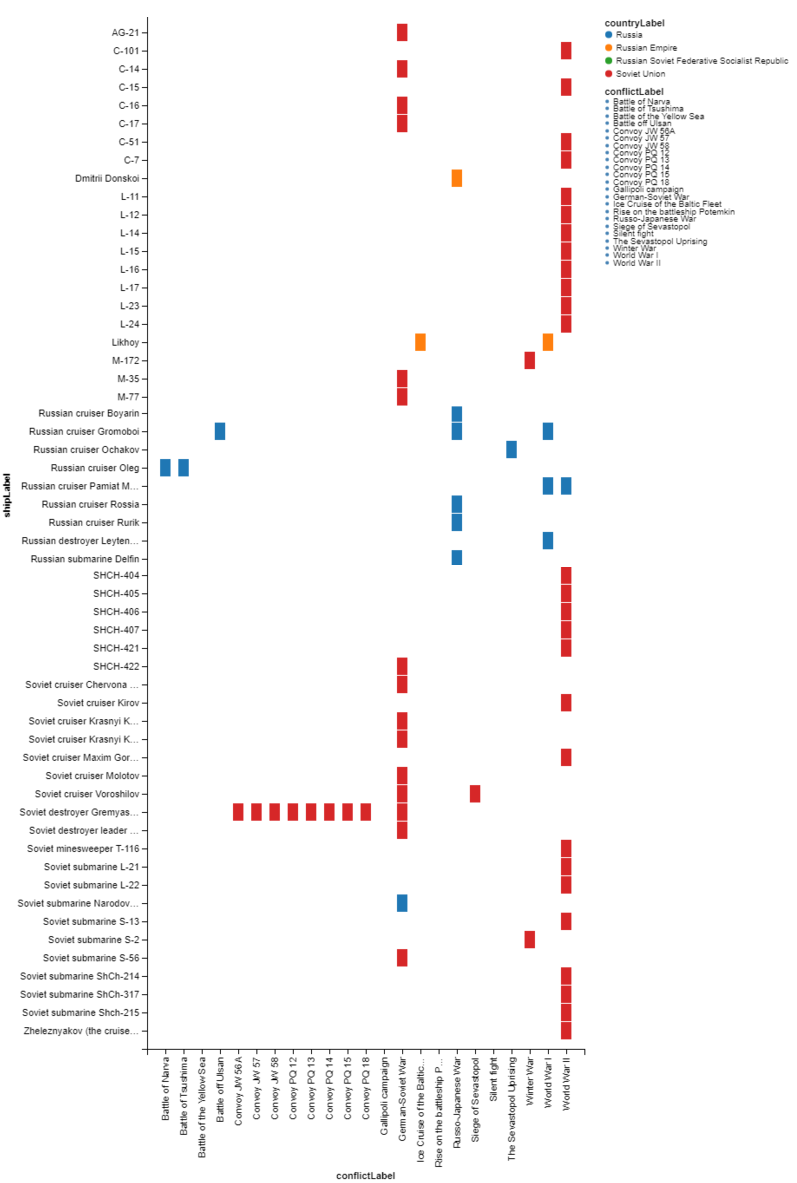
\includegraphics[width=0.95\linewidth]{chapter/ship/List_of_ships_with_countries_and_war_conflicts_in_English.png}}%
  }
    \caption[List of ships with countries and war conflicts]{Fragment of the list of ships with countries and war conflicts (2017). The list shows that most of the ships are associated with Russia and the USSR, as well as with the Second World War or the German-Soviet War.}%
    \label{fig:ships_by_country_and_conflict}%
\end{figure*}